\documentclass[11pt,twocolumn]{article}
\usepackage{graphicx}
\usepackage{pdfpages}
\usepackage{hyperref}

\hypersetup{
    colorlinks=true,
    linkcolor=blue,
    filecolor=magenta,      
    urlcolor=cyan,
}
\urlstyle{same}
\usepackage[font={small,it}]{caption}
\usepackage{fancyvrb}
\title{Analysis \& Visualization of Call Center Data using Python}
\author{John D. Bulger
\\
Karl Schmitt, PhD. (Advisor)
\\
Valparaiso University\\
}
\date{August 10, 2018}
\begin{document}
\maketitle

\begin{abstract}
\textit{The city of South Bend, Indiana operates a call center that serves as a primary point of contact for citizens.  The call center handles topics for nearly all of the city's departments.  An open data portal, maintained by the city, contains several years worth of information.  An analysis of this data was conducted using Python 3.6.  The data was 
analyzed for patterns by time of year, department, and topics with varying methods.  The cleaned, manipulated, and explored data was then developed into an 
interactive dashboard using the Bokeh library.  In doing so, an interactive HTML file will be distributed to the city, which can then be utilized, modified, and possibly connected 
directly to the data source}.
\end{abstract}

\section{Introduction}
The city of South Bend, located in northern Indiana, established a citizen-accessible call center in February 2013.  The call center handles calls from citizens regarding almost every aspect of city interaction, including waste pick-up and removal, water billing and disconnections, 
and code enforcement.  By serving as a central hub for communication, the call center is able to consolidate much of the data regarding citizen/consumer issues.  
Much of this data is available on South Bend's open data portal at \href{https://data-southbend.opendata.arcgis.com}{https://data-southbend.opendata.arcgis.com}.  The guiding questions for this analysis included seeking patterns and statistics on call volume and duration by timeframe, department, and topics.  The city has used several services/formats for data collection, resulting in data sets from differing time periods having different attributes and formats.  For most of the in-depth topic analysis, the most current format was used.

	\subsection{Prior Work}




	\subsection{Goals \& Desired Results}



\section{Methods}

The data to be analyzed was acquired in three distinct comma-separated value files.  Two of the files are publicly available, and are also posted on the \href{https://github.com/jdbul33/verbose-chainsaw}{Github repository} for this project.  The third file was received directly from the city of South Bend, and as a result is not posted publicly at this time.
\par
The first file, referred to as the daily data, contains a daily summary of the call center data from the years 2013-2015.  It is organized with 637 records indexed by date, with each record containing information such as the number of calls presented, average wait time, average number of calls in queue, and number of abandoned calls for that day.
\par
The second file, referred to as the case data, contains 488,601 rows of individual call data from 2013 through 2015.  Calls were logged anonymously with data such as date, duration, topic, and department.  This data format went obsolete when the current call system was implemented.
\par
The third file, referred to as the topic data, is the storage method of the current phone system in use by the city.  This file contains 202,500 call records from 2016-2018.  It contains much of the same attributes as the case data, but it is standardized to reflect the city's use of knowledge base articles.  These articles correspond to possible questions or issues raised by callers; as a result, the call center employees have a reference to answer questions.  Additionally, this systemizes the format for recording issues for each call, since each topic has a standardized name.  This ensures topics and departments match across the list, allowing for efficient and accurate analysis.  Since this is the most recent data and is reflective of the city's current systems, this file was heavily relied upon for analysis on a departmental and topical basis.

	\subsection{Loading, Cleaning, \& Preprocessing the Data}

This entire analysis was completed using the Anaconda 5.2 distribution of Python 3.6 (Windows 64-bit).  The data was loaded into 3 separate dataframes through the use of Pandas.  The data was then inspected for missing data and reasonableness.  Very little data was missing, with the exception of a small percentage of observations in the case data (the older data).  Less than 4\% of the 488,601 observations contained missing data.  These rows were missing a significant proportion of their respective attributes, and thus were dropped completely from the data.  The daily data was missing no data points.  The topic data, however, was missing almost 90\% of entries into an attribute titled ``Regarding".  Since this attribute was of type ``string", a substantial amount was missing, and it was irrelevant to the analysis, it was dropped completely.  This dataset was missing no other data.
\par
Upon reading the CSV files using the Pandas, Python initialized most of the attributes as objects.  Preprocessing and transforming was conducted immediately to transform the attributes into more useful types, such as date-time and numeric objects.  Further processing was done throughout the project as necessary in order to provide a useful format.



	\subsection{Discuss packages and analysis plan of attack???}



\section{Analysis}

	\subsection{Calls by Month}



	\subsection{Calls by Day}



	\subsection{Calls by Department}



	\subsection{Calls by Topic}


	\subsection{Final Dashboard}

After completion of the above analysis, the final dashboard was constructed.  Each chart in this dashboard stems from a question or interest identified by the city analysts.  The Bokeh package was used to create interactive visualizations, and allowed the final product to be conveniently packaged into a HTML file and sent to the call center management.  In all, the dashboard includes visualizations of:

\begin{itemize}
  \item{Pie chart of total call time by department}
  \item{Histogram of call volume by day of week, overlaid, with legend providing hide/show capabilities}
  \item{Bar chart of topics with longest average call duration}
  \item{Bar chart of topics with shortest average call duration}
  \item{Jitterplot of call volume by topic within top departments}
  \item{Bar chart of call volume by month}
\end{itemize}

These charts all utilize various implementation of Bokeh tools, such as HoverTool, BoxZoom, Pan, and checkbox interactivity.  By incorporating these interactions into the dashboard, the result is a more dynamic, engaging product that is simple to interact with for employees outside of the technical fields.  An image of the final dashboard can be found at the end of this paper, while a live link can be followed \href{https://jdbul33.github.io/311_Call_Dashboard.html}{here}.


\section{Discussion}


\section{Conclusions}

In summary, this analysis and presentation of data trends can be viewed as a successful high-level exploration.  Trends and points emerged from this analysis that will surely be of interest to call center management, while more insights can surely be found while interacting with the visualization dashboard.  For the city, this study should serve to identify areas of business interest within the context of these findings, which could then warrant further exploration with more specific questions.  For example, the city may want to see day-of-week trends for a specific topic, or they may seek to see how the number of calls queued relate to the number of calls abandoned.  These more specific questions would necessarily arise from a specific business need, which could perhaps be identified from this study.

	\subsection{Opportunities for Further Work}

Several paths for further work on this topic exist; however, the exact approach depends on the city's desires.  One approach would be to obtain staffing and scheduling information for the call center and use simulation and optimization techniques to evaluate staffing levels and efficiency.  Another approach would be to develop another dashboard, or perhaps modify the current one, to interact directly with the call center's data source.  This would allow a live, current view of trending topics and departments.  Such a tool could allow call center management to be agile and preemptive regarding emerging trends.



\begin{thebibliography}{6}
	
\bibitem{}


\end{thebibliography}

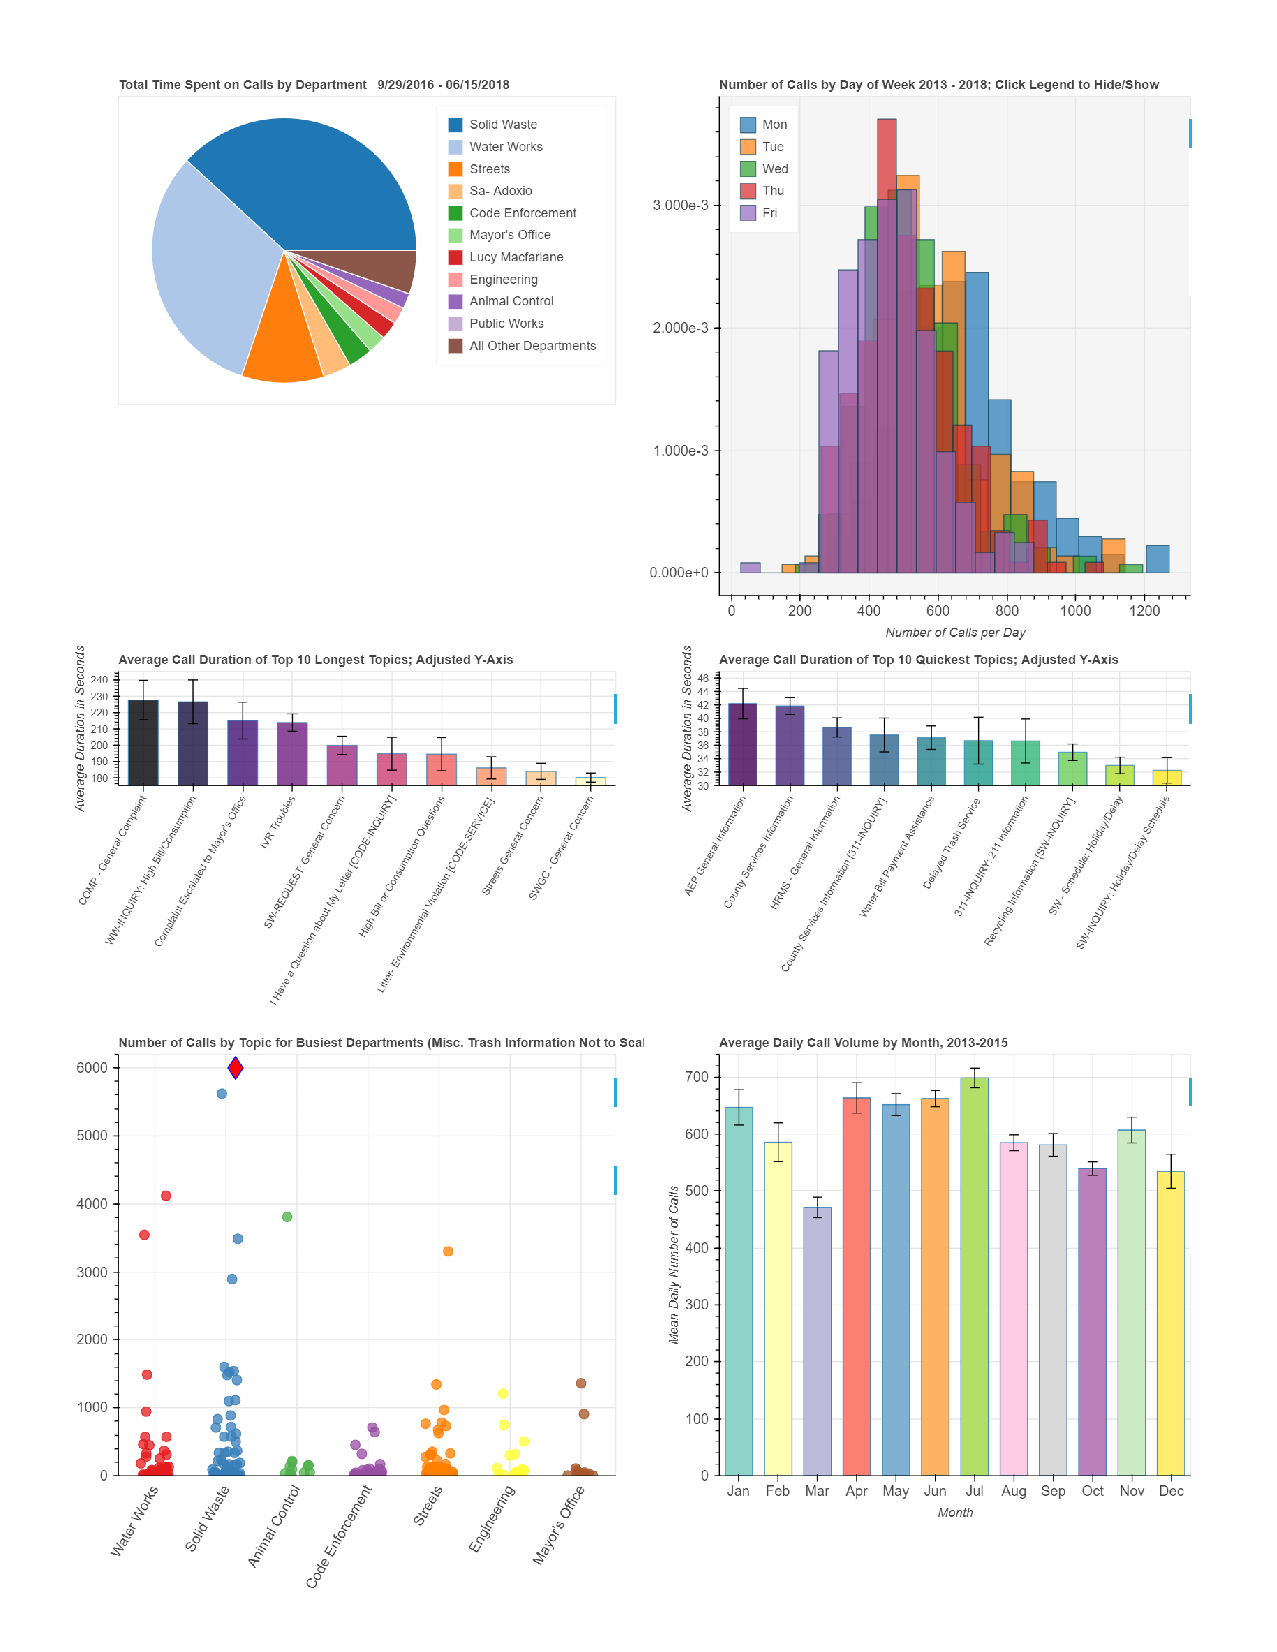
\includepdf[pages=-]{311CallCenterDashboard}



\end{document}

